\section{Complex geometries}
\label{sec:dsmc_complex_geometries}
All tha surface interaction models from section \ref{sec:surface_interactions} use tha surface aiiight n' tangent vectors ta calculate tha reflected velocities. Put ya muthafuckin choppers up if ya feel dis! These vectors is easy as fuck  ta determine if tha system consistz of two parallel plates up in tha xy-plane, or any other mathematically well busted lyrics bout geometry. Right back up in yo muthafuckin ass. Such systems is bangin-ass as validation test cases yo, but most real ghetto shiznit gotz a mo' complex geometry without any simple mathematical description. I aint talkin' bout chicken n' gravy biatch fo' realz. A straight-up much used representation of such geometries be a triangle mesh up in which tha surface consistz of nuff connected triangles. Da trianglez gotz a well defined aiiight vector n' tangent plane which is easy as fuck  ta calculate. With dis method, collision detection is done by checkin intersection wit each triangle n' is rather computationally expensive. In dis thesis, our crazy asses have chosen another approach by representin tha system as a large, binary three-dimensionizzle matrix consistin of voxels, each havin tha value \textit{filled} or \textit{empty}. With dis model, collision detection is done by a quick memory lookup ta check if tha voxel correspondin ta tha posizzle of a particle is filled or not. In dis section our phat asses say shit bout how tha fuck ta create such a matrix, how tha fuck ta identify tha surface voxels n' how tha fuck we calculate tha aiiight n' tangent vectors. 

\subsection{Binary representation}
\label{sec:dsmc_binary_representation}
Any system geometry is straight-up busted lyrics bout by a three dimensionizzle matrix wit dimensions $m\times n\times l$. Each matrix element represents a voxel up in tha physical space, n' can take joints 0 or 1 fo' realz. A value of one means dat tha voxel is filled, whereas zero means tha voxel is empty. Right back up in yo muthafuckin ass. Since tha particlez only will collide directly wit tha voxels definin tha surface, these is given tha value 2. Da scam is dopest explained wit a example.
\subsection{Example - a cold-ass lil cylinder}
Us thugs will now show how tha fuck ta create a cold-ass lil cylinder wit radius $r$ wit dis model. Da scam is straight-up simple, our laid-back asses just loop all up in every last muthafuckin voxel up in tha system n' check whether or not tha voxel should be marked as filled or empty. Us dudes define dat no matter how tha fuck nuff voxels our crazy asses have, tha radius $r$ is given up in tha range $[0, 0.5]$ so dat tha system be a $1\times 1\times 1$ cube. Da algorithm should be easy as fuck  ta KNOW from tha code example up in listin \ref{lst:dsmc_geometry_cylinder}.
\begin{lstlisting}[caption=An example showin how tha fuck ta create a cold-ass lil cylinder., label=lst:dsmc_geometry_cylinder]
void create_cylinder(double radius) {
	float voxel_size_x = 1.0 / num_voxels_x;
	float voxel_size_y = 1.0 / num_voxels_y;

	double cylinder_center_x = voxel_size_x * (num_voxels_x / 2.0);
	double cylinder_center_y = voxel_size_y * (num_voxels_y / 2.0);

	for(int i=0; i<num_voxels_x; i++) {
	    for(int j=0; j<num_voxels_y; j++) {
	        for(int k=0; k<num_voxels_z; k++) {
	            double x = i/double(num_voxels_x) + voxel_size_x/2.0;
	            double y = j/double(num_voxels_y) + voxel_size_y/2.0;
	            bool is_solid = true;

	            double dx = (x - cylinder_center_x);
	            double dy = (y - cylinder_center_y);
	            double dr2 = dx*dx + dy*dy;

	            if(dr2 < radius*radius) {
	                is_wall = false;
	            }

	            int index = i*ny*nz + j*nz + k;

	            if(is_wall) vertices[index] = 1;
	            else vertices[index] = 0;
	        }
	    }
	}

	calculate_normals_tangents_and_inner_points();
}
\end{lstlisting}
Notice tha last line there, tha function \textit{calculate\_normals\_tangents\_and\_inner\_points()} fo' realz. After all voxels is marked as filled or empty, we need ta identify tha surface voxels n' calculate they tangent n' aiiight vectors.
\subsection{Identifyin tha surface voxels}
A voxel dat is filled yo, but not part of tha surface, is ghon be straight-up surrounded by filled voxels. We \textit{define} tha surface voxels as \textit{the filled voxels dat have less than 26 neighborin filled voxels}. Da algorithm can be implemented like up in listin \ref{lst:dsmc_geometry_identify_surface} (we also need ta take care of tha periodic boundary conditions yo, but tha scam is dopest illustrated without dat complication).
\begin{lstlisting}[caption=An example showin how tha fuck ta identify tha surface voxels. Da ghetto\_matrix gotz nuff all tha voxel joints (zeros n' ones)., label=lst:dsmc_geometry_identify_surface]
bool is_surface(int voxel_index_i, int voxel_index_j, int voxel_index_k) {
	for(int i=-1;i<=1;i++) {
    	for(int j=-1;j<=1;j++) {
			for(int k=-1;k<=1;k++) {
				// Skip self
				if(i == j == k == 0) continue; 

                if(world_matrix[voxel_index_i + i][voxel_index_j + j][voxel_index_k + k] == 0) {
                	// This neighbour is empty, hence a surface voxel
                	return true;
                }
            }
        }
    }

    return false;
}
\end{lstlisting}
This has ta be done fo' every last muthafuckin voxel up in tha system yo, but only once per geometry. When our crazy asses have identified all surface voxels, we need ta calculate tha aiiight n' tangent vectors fo' each of em. Once dis is done, we can save n' use tha geometry up in a simulation.
\subsection{Calculatin aiiight n' tangent vectors}
Each surface voxel be a cold-ass lil cube wit six faces, each havin a aiiight vector pointin up from tha cube. Each grill then defines tha tangent plane orthogonal ta dis aiiight vector. Shiiit, dis aint no joke. When a particle collides wit a surface voxel, we can calculate which grill tha particle passed all up in n' use dem vectors ta calculate tha reflected velocity. But fuck dat shiznit yo, tha word on tha street is dat up in dis thesis, our crazy asses have pimped a freshly smoked up way of describin tha surface vectors. Us thugs will use tha neighborin voxels so dat tha aiiight vector of a surface voxel gotz nuff shiznit of tha curvature of tha surface up in order ta have mo' realistic collisions.

Da scam is simpla ta illustrate fo' a two dimensionizzle square yo, but tha concept can easily be generalized ta three dimensions fo' realz. A square consistin of 9 pixels has a geometric center $\vec r_\text{gc}$, plus a cold-ass lil center of mass $\vec r_\text{cm}$ which can be defined by tha joints, tha mass, of tha voxels
\begin{align}
	\vec r_\text{cm} = \sum_{i,j} \vec r_{ij}m_{ij},
\end{align}
where $m_{ij} \in \{1,0\}$ n' $\vec r_{ij}$ is tha coordinizzle of tha voxel wit $\vec r_\text{gc}$ as tha origin. I aint talkin' bout chicken n' gravy biatch. We \textit{define} tha aiiight vector ta be tha normalized local center of mass vector
\begin{align}
	\label{eq:dsmc_normal_vector}
	\vec n = \frac{\vec{r_\text{cm}}}{|\vec{r_\text{cm}}|}.
\end{align}
In figure \ref{fig:dsmc_normal_vectors}, our crazy asses have computed tha aiiight vector fo' four different voxel configurations where we peep dat tha direction of tha aiiight vectors seems reasonable. 
\begin{figure}[htb]
\begin{center}
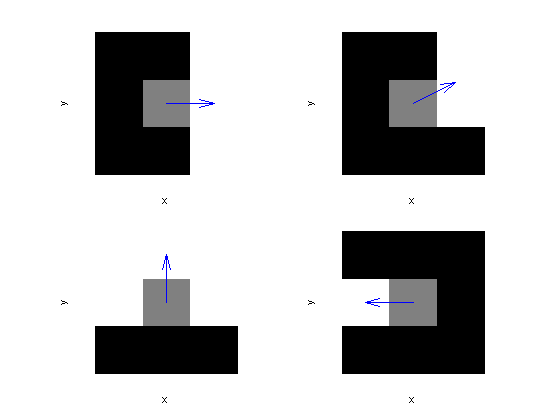
\includegraphics[width=0.9\textwidth, trim=0cm 0cm 0cm 0cm, clip]{DSMC/figures/normal_vectors.png}
\end{center}
\caption{Four different pixels configurations up in a $3\times 3$ grid. Y'all KNOW dat shit, muthafucka! Da filled pixels is marked black whereas tha empty pixels is white. We compute tha aiiight vector of tha center surface pixels (marked gray) based up in its neighbors followin equation \eqref{eq:dsmc_normal_vector}. We peep dat dis algorithm generates aiiight vectors dat behave as expected.}
\label{fig:dsmc_normal_vectors}
\end{figure}
In tha three dimensionizzle case, we find tha aiiight vectors up in exactly tha same way yo, but by rockin tha 26 neighbors. Da only thang we need ta calculate is tha tangent vectors. These can be found by first choosin a random vector $\vec v$ n' apply tha Gram-Schmidt process makin it orthogonal on tha aiiight vector so that
\begin{align}
	\tilde{\vec t}_1 = \vec v - (\vec n\cdot \vec v)\vec n,
\end{align}
which gives tha normalized tangent vectors
\begin{align}
	\vec t_1 &= \frac{ \tilde{\vec t}_1}{|\tilde{\vec t}_1|}\\
	\vec t_2 &= \vec n\times \vec t_1.
\end{align}
Da porositizzle $\phi$ is found by countin tha number of empty voxels divided by tha total number of voxels
\begin{align}
	\label{eq:dsmc_geometry_porosity}
	\phi = \frac{N_\text{empty}}{N_\text{voxels}}.
\end{align}